\documentclass[11pt, a4paper]{article}

\usepackage{amsmath}
\usepackage{amsfonts} %Matheschriften
\usepackage{amssymb} %Mathesymbole
%\usepackage{mathptmx} % Einstellung für Schriften und Sonderzeichen in mathematischen Umgebungen
                        % ändert SChriftfont
\usepackage{wasysym} % Stellt diverse Sonderzeichen bereit
\usepackage{siunitx}
\usepackage{float}
\usepackage{microtype}
\usepackage{graphicx}
\usepackage{hyperref}
\usepackage{xcolor}
\usepackage[section]{placeins}
% allows for temporary adjustment of side margins
\usepackage{changepage}
\usepackage{rotating}


\usepackage[ngerman]{babel}
\addto\captionsngerman{%
 \renewcommand{\abstractname}{Einleitung}}

\title{Versuch 4: Magnetismus}
\author{Team 2-13: Jascha Fricker, Benedict Brouwer}

\begin{document}
    \maketitle

    \tableofcontents

    \newpage

    \section{Einleitung}

    In diesem Versuch werden die Eigenschaften des Magnetfelds einer Spule mittels einer Hall-Sonde untersucht. Dabei wird der Einfluss verschiedener Ströme und eines Metallkerns gemessen.

    \section{Theorie}

    Nach dem Biot-Savart-Gesetz kann das Magnetfeld $B(x)$ auf der Symmetrieachse einer dünnen Ringspule mit Radius $R$ durch die Formel
    \begin{align}
        B(x) = \frac{\mu_0 \mu_r N}{2} \cdot \frac{R^2 I}{\left(x^2 + R^2\right)^{\frac{3}{2}}} \label{eq:BiotSavart}
    \end{align}
    beschreiben werden. Dabei durchfließt die Spule eine Stromstärke $I$ mit einer Windungszahl $N$. Das Material in der Spule hat eine Permeabilität $\mu_r$ (bei Luft $\mu_r = 1$).
    
    Durch Umstellung der Gleichung nach $x$ können bei gegebenem $B_{max}$ die Spulenränder
    \begin{align}
        x_{min, \ max} = \pm \sqrt{\left(\frac{\mu_0 \mu_r N}{2} \cdot \frac{R^2 I}{B_{max}}\right)^\frac{2}{3} - R^2} \label{eq:bmax}
    \end{align}
    bestimmt werden.
    
    Wenn ein Material in das Spuleninnere gegeben wird, kann das Magnetfeld innerhalb der Spule $B_M$ durch das Magnetfeld $B_0$ ohne Material und die magnetische Permeabilität $\mu_r$ berechnet werden
    \begin{align}
        B_M = \mu_r \cdot B_0 \,. \label{eq:B_M}
    \end{align}
    Außerdem kann die Magnetisierung
    \begin{align}
        M = \chi_m \cdot H = (\mu_r - 1) \cdot \frac{B_0}{\mu_0} \,. \label{eq:magnet}
    \end{align}
    berechnet werden.
    \section{Versuchsaufbau und Druchführung}
    Zur Untersuchnug der magnetischen Eigenschaften einer Spule wurde auf einem linear verschiebbaren Schlitten zwei verschiedene Hallsonden mit jeweils unterschiedlicher Ausrichtung montiert.
    Mit diesen wurde mit variierendem Abstand zur Spule die magnetische Flussdichte gemessen. Es wurde das B-Feld in longditudinaler Richtung bei 1 \si{\ampere}, 1.5 \si{\ampere} und bei 1 \si{\ampere} mit Metallkern gemessen.
    Des Weiteren wurde das B-Feld in Transversalrichtung bei 1 \si{\ampere} gemessen.
    \section{Ergebnisse und Diskussion}
    \subsection{longitudinale Konfiguration}
    Die rohen Messwerte der verschiedenen Messreihen der longitudinalen Konfiguration wurden im Graph \ref{fig:longmessohneKern} (ohne Metallkern) und \ref{fig:longmessmitKern} (mit Metallkern) geplottet.
    \begin{figure}[h]
        \centering
        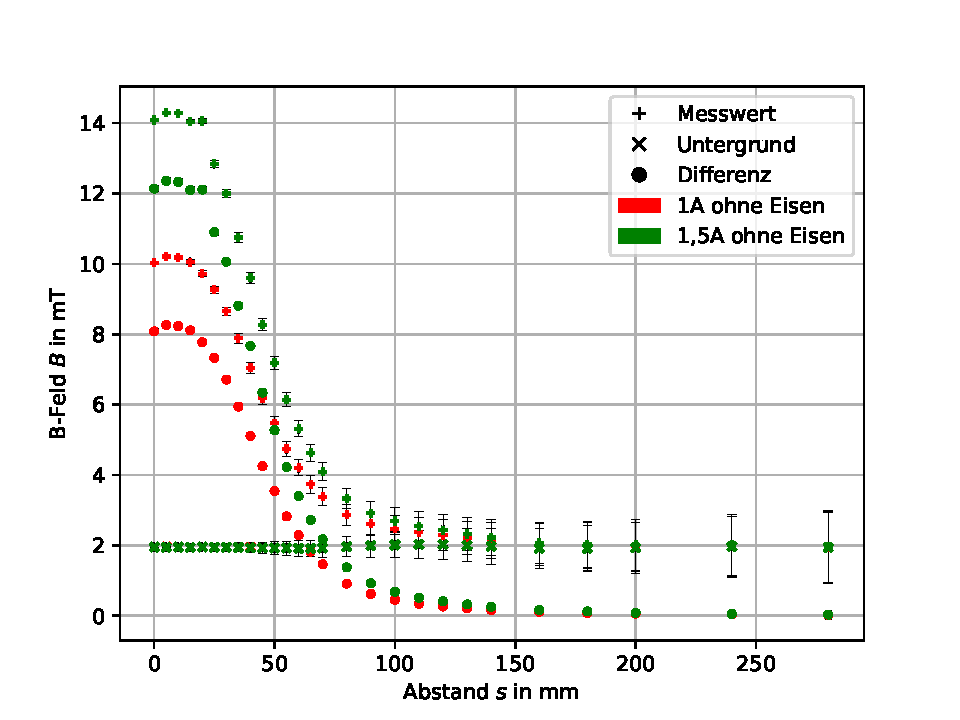
\includegraphics[width=0.9\textwidth]{ohneKernRaw.pdf}
        \caption{Messwerte der longitudinalen Konfiguration ohne Metallkern}
        \label{fig:longmessohneKern}
    \end{figure}

    \begin{figure}[h]
        \centering
        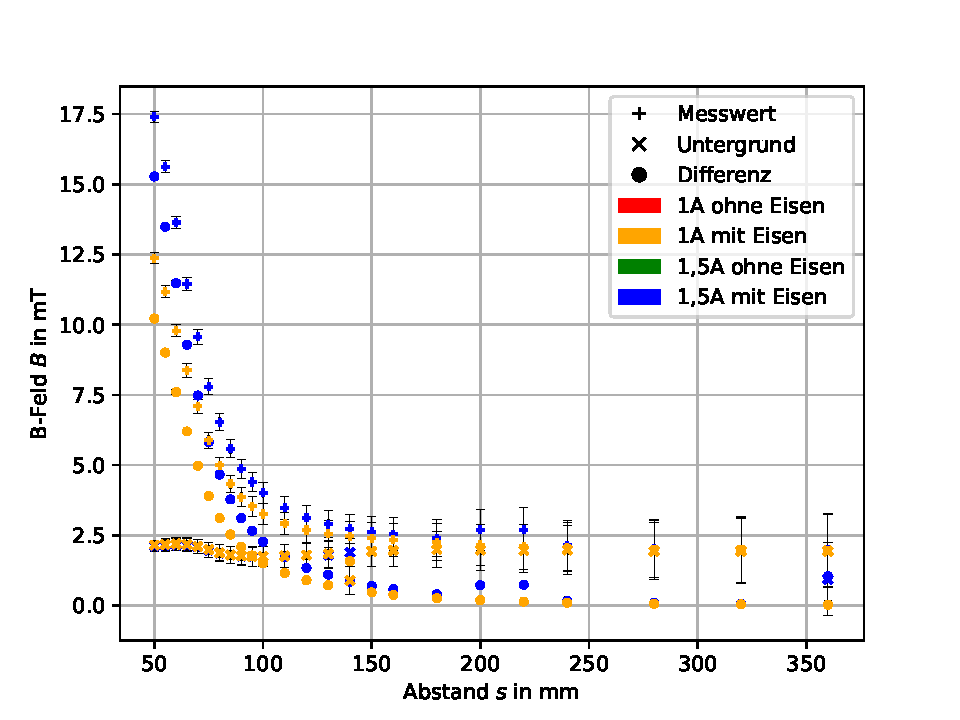
\includegraphics[width=0.9\textwidth]{mitKernRaw.pdf}
        \caption{Messwerte der longitudinalen Konfiguration mit Metallkern}
        \label{fig:longmessmitKern}
    \end{figure}
    \begin{figure}[h]
        \centering
        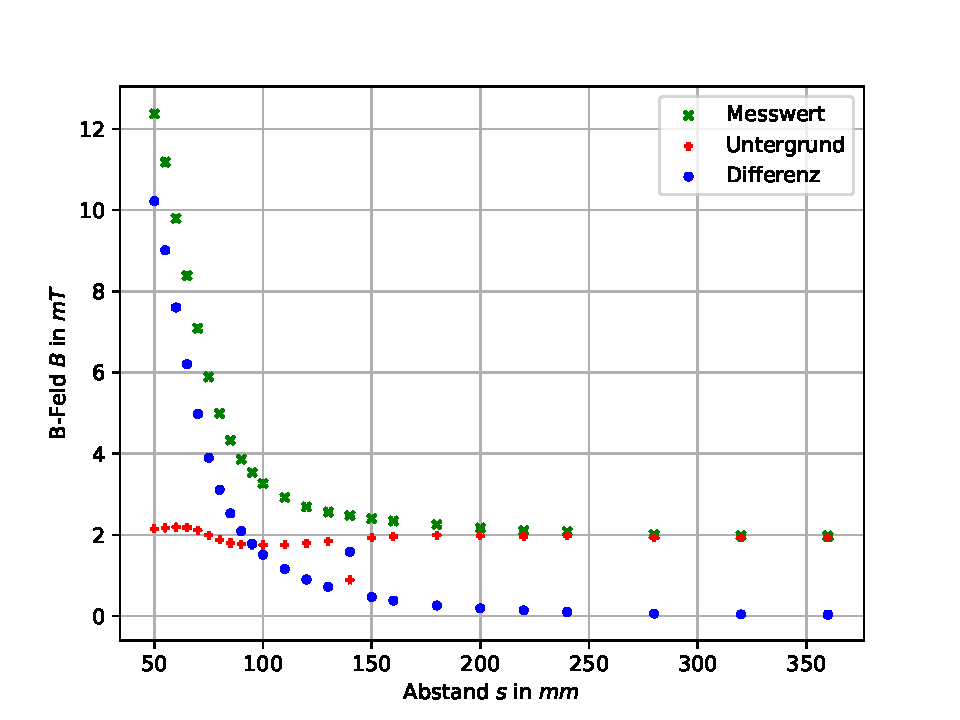
\includegraphics[width=0.8\textwidth]{raw2.pdf}
        \caption{Messwerte transversale Konfiguration}
        \label{fig:transmess}
    \end{figure}



    Im Plot \ref{fig:longfit1a} (longditudinale Konfiguration $1 \si{\ampere}$) wurde die magnetische Flussdichte abzüglich der Hintergrundmagnetisierung aufgetragen und gespiegelt. Anschließend wurde die Funktion (\ref{eq:BiotSavart}) auf die Messwerte außerhalb der Spule gefittet und auch aufgetragen. Mit einem abgelesenen $B_{max}$,  den gefitteten Parametern und der Funktion (\ref{eq:bmax}) wurden die Spulenränder berechnet. Diese werden als vertikale Balken in dem Graphen dargestellt. 
    Die Ergebnisse des Fits und die errechneten Werte sind in Tabelle \ref{tab:fit} aufgelistet. Für den Fit wurden I und R als Fitparameter verwendet, da diese von den gemessene Werten bei der Versuchsdurchführung abweichen. Dies liegt an der Erwärumung der Spule und da die Spule nicht, wie in der Theorie angenommen, rund ist.
    Die gleiche Auswertung der Messreihe mit 1,5A Stromstärke ist im Graph \ref{fig:longfit15a} dargestellt.
    
    Bei beiden Messreihen ist es erstaunlich, wie stark $I_{\text{eff}}$ von der eingestellten Stromstärke abweicht. Die Abweichung ist aber bei beiden Messreihen in sich konsistent. Auch der gefittete Radius $R_{\text{eff}}$ ist bei beiden Messreihen konsistent. Nur die Länge der Spule ist bei unterschiedlich. Dies kann aber auch daran liegen, dass die Abweichungen vom Biot-Savart-Gesetz mit der Stromstärke skalieren, und so der homogene Bereich des Magnetfeldes größer wird.
    \begin{table}[h]
        \centering
        \begin{tabular}{c | c | c}
            \textbf{Parameter} & \textbf{Wert mit 1A} & \textbf{Wert mit 1,5A} \\
            \hline
            $B_{max}$ & $8,26(41) \si{\milli\tesla}$ & $12,4(55) \si{\milli\tesla}$ \\
            $R_{eff}$ & $35,6(10) \si{\milli\metre}$ & $35,8(11) \si{\milli\metre}$ \\
            $I_{eff}$ & $0,739(16) \si{\ampere}$ & $1,098(25) \si{\ampere}$ \\
            $x_{min}$ & $25,9(54) \si{\milli\meter}$ & $25,8(55) \si{\milli\meter}$ \\
            $x_{max}$ & $-25,9(54) \si{\milli\meter}$ & $-25,8(55) \si{\milli\meter}$ \\
        \end{tabular}
        \caption{Ergebnisse Aufgabe 5.2.2}
        \label{tab:fit}
    \end{table}

    \begin{figure}
        \centering
        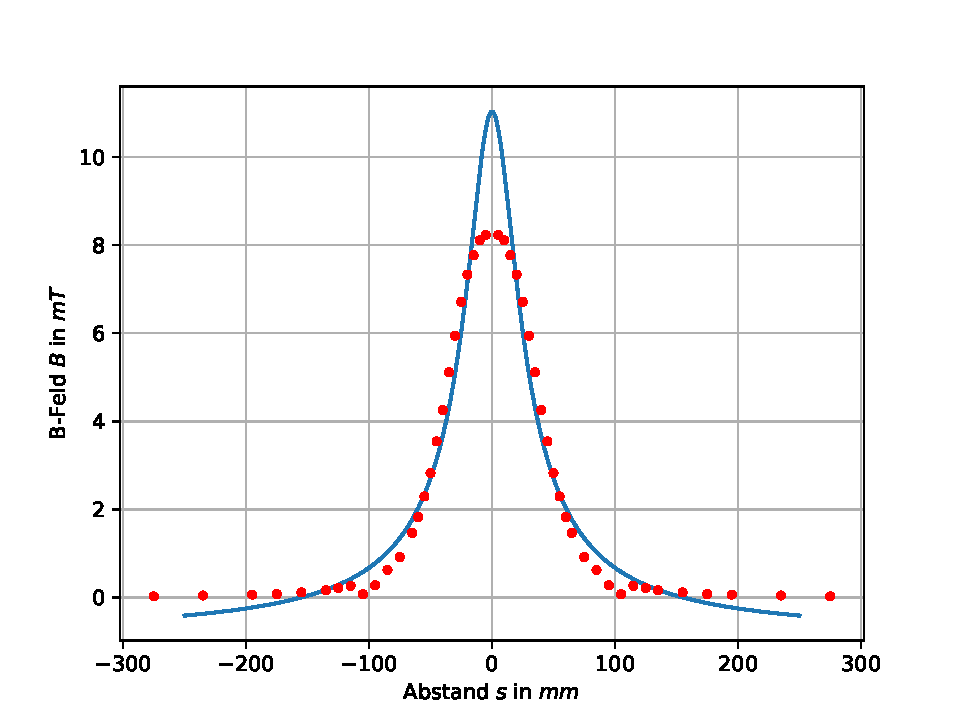
\includegraphics[width=0.8\textwidth]{fit1.pdf}
        \caption{Fit der longitudinalen Konfiguration bei 1 Ampere}
        \label{fig:longfit1a}
    \end{figure}

    \begin{figure}
        \centering
        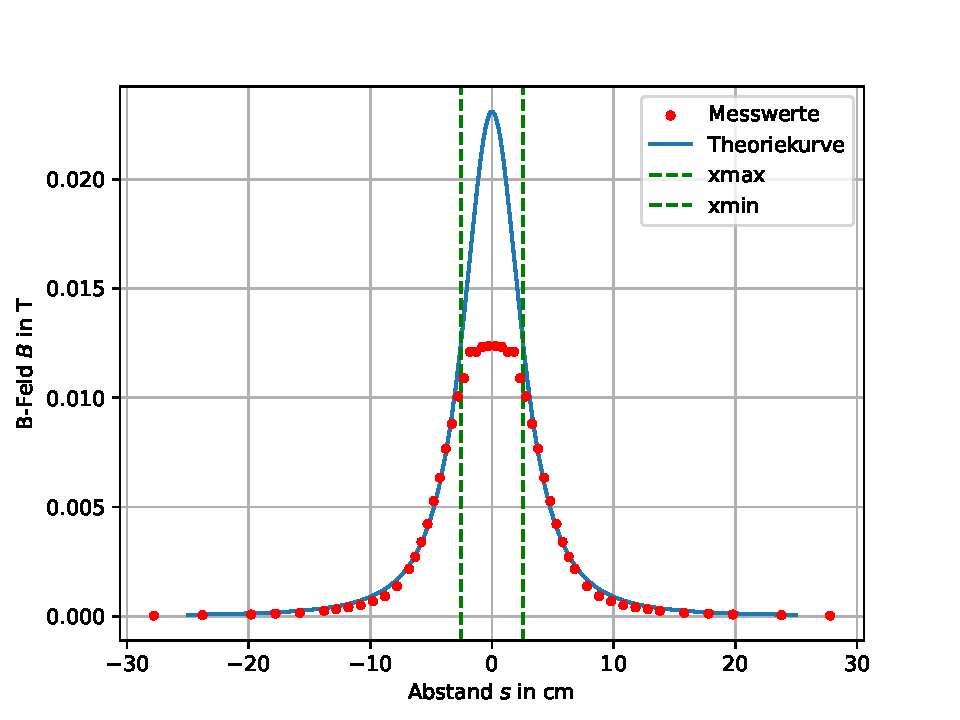
\includegraphics[width=0.8\textwidth]{fit15a.pdf}
        \caption{Fit der longitudinalen Konfiguration bei 1,5 Ampere}
        \label{fig:longfit15a}
    \end{figure}

    \subsection{Bestimmung von $\mu_r$}
    Mit den in Tabelle \ref{tab:fit} aufgelisteten Ergebnissen, kann die Funktion \ref{eq:BiotSavart} mit einem freien Parameter $\mu_r$ auf die Messwerte der longitudinalen Konfiguration gefittet werden (Siehe Abb. \ref{fig:murfit}). So kann 
    \begin{align}
        \mu_r = 2.6469(63)
    \end{align} bestimmt werden.
    
    Dies ist eine relative Permeabilität die man eigentlich paramagnetischen Stoffen zuordnen würde. Allerdings lässt die vergleichsweise geringe magnetische Flussdichte vermuten, dass es sich um einen ferromagnetischen Stoff handelt, der seine charakteristischen Weißschen Bezirke nicht voll umfänglich ausbilden konnte.
    Was dazu führt, dass die tasächlich gemessene relative Permeabilität weit von dem entfernt ist, was für ferromagnetische Stoffe üblich ist.
    %Daraus folgt, dass es sich um einen stark paramagnetischen Stoff handelt, der vermutlich ein Legierung aus einem ferromagnetischen Stoff wie Eisen und einem paramagnetischen Stoff wie z.B. Magnesium ist.
    
    
    Nun kann die Magnetisierung der Spule mit Metallkern mittels Gleichung (\ref{eq:magnet}) und die maximale magnetische Flussdichte der Spule mittels Gleichung (\ref{eq:B_M}) berechnet werden.
   \begin{align}
        B_{M} = 21,8(13) \si{\milli\tesla} \\
        M = 10,77(75) \si{\kilo\ampere\per\metre}
    \end{align}
    \begin{figure}
        \centering
        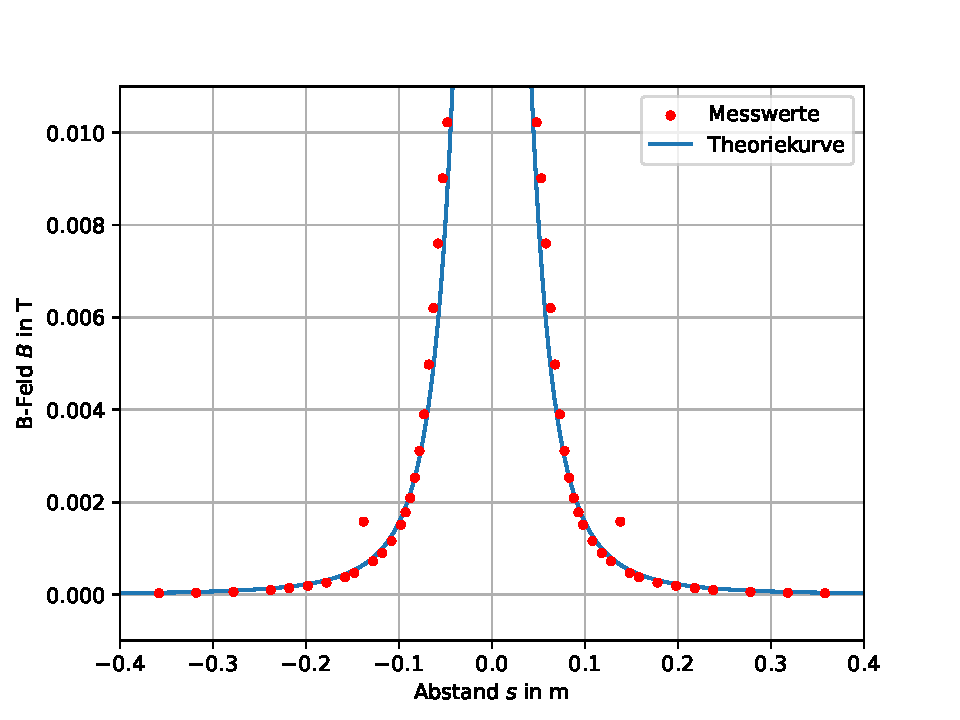
\includegraphics[width=0.8\textwidth]{mur.pdf}
        \caption{Fit der Permeabilitätsmessung}
        \label{fig:murfit}
    \end{figure}

    \subsection{transversale Konfiguration}
    Die gemessenen Daten der transversalen Konfiguration wurden mit den Daten der longditudinalen Messung im Graph \ref{fig:LogVergleich} geplottet.
    Dabei fällt auf, dass die Magnetfelder auf mit ähnlichem Kurvenverlauf abfallen welcher aber logarithmisch um einen festen Wert verschoben ist.
    Erstaunlicherweise ist der Startwert der transversalen Messung mit $10 \si{\milli\tesla}$ direkt an der Seite der Spule größer als der Wert der longitudinalen Messung direkt in der Spule, der etwa $8 \si{\milli\tesla}$ beträgt.
    \begin{figure}[h]
        \centering
        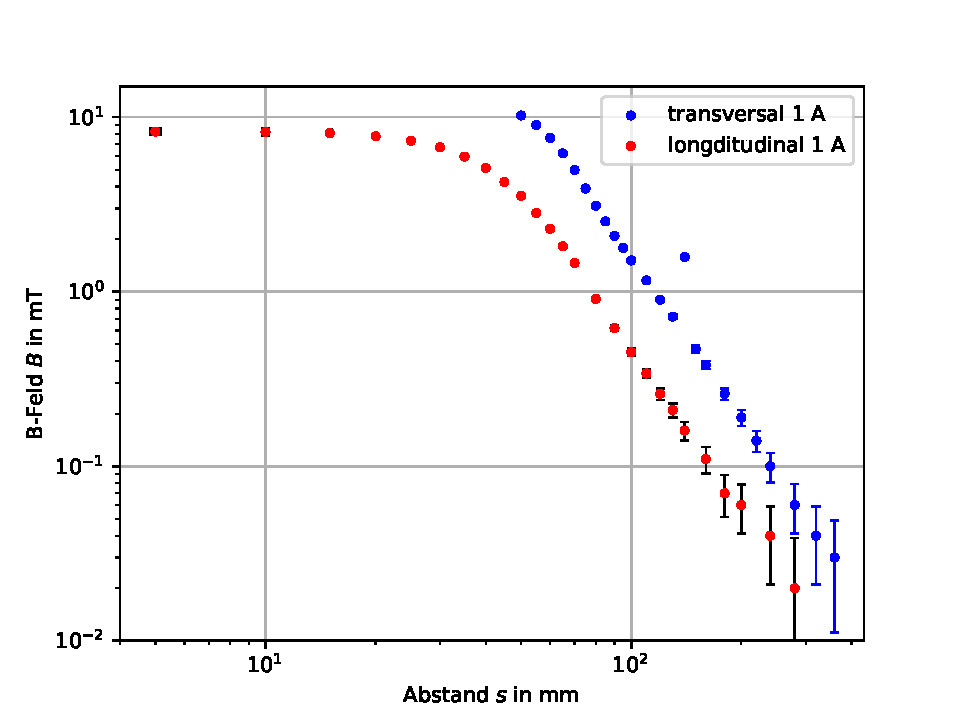
\includegraphics[width=0.8\textwidth]{logarithmischerVergleich.pdf}
        \caption{Vergleich der transversalen und longditudinalen Messkonfiguration}
        \label{fig:LogVergleich}
    \end{figure}





    \section{Anhang}
    \subsection{Gaußsche Fehlerfortpflanzung}
    Die Fehlerfortpflanzung wurde mithilfe der Formel
    \begin{align}
        u\left(g \left(x_1, ..., x_n\right)\right) = \sqrt{\sum_{i=1}^n \left( \frac{\partial g }{\partial x_i} \cdot u\left(x_i\right) \right)^2} \label{gauss}
    \end{align}
    berechnet.
    \bibliographystyle{plain}
    \bibliography{literature}

\end{document}